\section{Lezione 12 - Support Vector Machine}\label{lezione-12---support-vector-machine}

\textbf{Richiamo}: l'errore \textbf{ideale}, cioè quello commesso su esempi che
non sono stati valutati durante l'apprendimento, può essere visto come
composto da due termini, un errore empirico sui dati e la VC-Confidence.

L'algoritmo di minimizzazione dei rischi cerca lo spazio delle impotesi
che va a minimizzare la VC-Confidence.

\subsection{SVM - Idea di base}\label{svm---idea-di-base}

Sappiamo che la VC dimension di un iperpiano nello spazio \emph{m} è
\emph{m+1}.

Considerando il caso in cui gli esempi sono linearmente separabili si
può definire il margine \emph{r} come la distanza minima tra l'iperpiano separatore
e l'esempio più vicino.

L'iperpiano che ha un margine maggiore viene detto ottimo e massimizza
la minima distanza con gli esempi.

\begin{figure}[htbp]
\centering
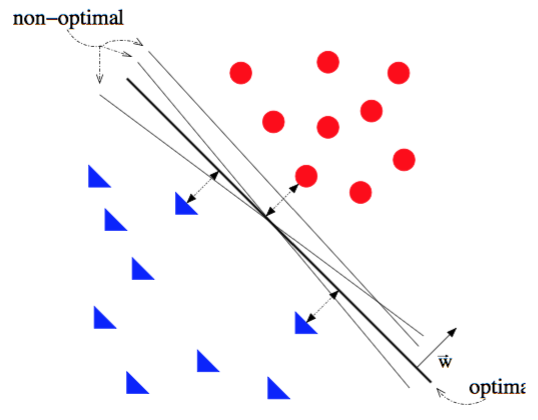
\includegraphics[width=0.4\textwidth]{./notes/immagini/l12-space.png}
\caption{Possibili iperpiani separatori}
\end{figure}

\subsubsection{Margine}\label{margine}

La distanza di un vettore da un iperpiano può essere misurata in modo algebrico.

Dato un iperpiano $\vec{w} \cdot \vec{x} + b = 0$, è possibile definire una funzione $g(\vec{x}) = \vec{w} \cdot \vec{x} + b$ che restituisce la distanza algebrica del vettore $\vec{x}$ dall'iperpiano.

Questo perché $\vec{x}$ può essere espresso come:

$$ \vec{x} = \vec{x}_p + r\frac{\vec{w}}{||\vec{w}||}$$

ovvero come somma tra la sua proiezione sull'iperpiano ($\vec{x}_p$) e il vettore perpendicolare all'iperpiano, scalato con la distanza dal punto ($r\frac{\vec{w}}{||\vec{w}||}$).

Considerando che $g(\vec{x}_p) = 0$ perché $\vec{x}_p$ è un punto dell'iperpiano, si ottiene:

\begin{align*}
g(\vec{x}) &= \vec{w} \cdot \vec{x} + b  \\
				  &=\vec{w}\cdot (\vec{x}_p + r\frac{\vec{w}}{||\vec{w}||}) + b \\
				  &=\vec{w}\cdot \vec{x}_p + b + \vec{w}\cdot r\frac{\vec{w}}{||\vec{w}||}  \\
				  &= r||\vec{w}||
\end{align*}

Per ottenere \textit{r} si può quindi utilizzare $r = \frac{g(\vec{x})}{||\vec{w}||}$ e dal momento che ci sono infinite soluzioni che differiscono solamente per un fattore di scala di $\vec{w}$, ci si limita al caso $r = \frac{1}{||\vec{w}||}$.

La distanza assoluta che c'è tra un punto classificato positivamente e un punto classificato negativamente dall'iperpiano risulta quindi essere $\rho = \frac{2}{||\vec{w}||}$.

\begin{figure}[htbp]
\centering
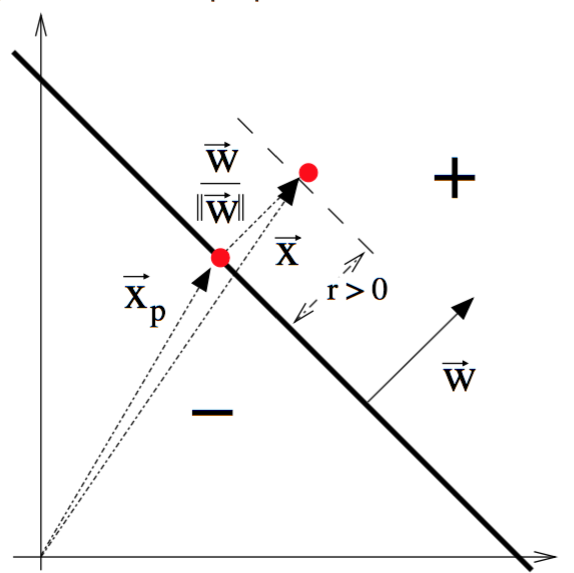
\includegraphics[width=0.4\textwidth]{./notes/immagini/l12-margine.png}
\caption{Margine}
\end{figure}

\subsubsection{Legame con SRM}

L'insieme degli iperpiani descritti dall'equazione $\vec{w} \cdot \vec{x} + b = 0$ possiede VC-Dimension:

$$ h \leq min\{\lceil \frac{R^2}{\rho^2}\rceil, m\} +1$$

dove $R$ è il diametro della palla più piccola che contiene tutti gli esempi di apprendimento.

Considerando lo spazio delle ipotesi

$$H_k = \{\vec{w} \cdot \vec{x} + b | \: ||\vec{w}||^2 \leq c_k\} \text{ con } c_1 < c_2 < \ldots$$

e assumendo di avere un insieme di dati linearmente separabili si riesce ad apprendere l'interno training set con errore empirico nullo.

L'approccio SRM (§\ref{sec:srm}) prevede quindi di selezionare lo spazio delle ipotesi con VC-Dimension minore (§\ref{sec:vcc}) ed in questo caso specifico consiste nel scegliere l'iperpiano che massimizza il margine di separazione $\rho$, ovvero che minimizza $||\vec{w}||^2$ .

\subsubsection{Alla ricerca dell'iperpiano ottimo}

Assumendo di avere $n$ esempi $\{(\vec{x}_i, y_i)\}$ \textbf{linearmente separabili} è possibile formulare un problema di ottimizzazione quadratica per trovare l'iperpiano ottimo che li separa:

$$ min_{\vec{w}, b} \frac{1}{2}||\vec{w}||^2 $$

$$ \text{s.t.: } \forall i \in \{1, \ldots , n\} : y_i(\vec{w} \cdot \vec{x}_i + b) - 1 \geq 0 $$

I vincoli rappresentano il fatto che gli esempi positivi ($y_i = 1$) vengano essere classificati come positivi e quelli negativi ($y_i = -1$) come negativi.

Dal momento che sia la funzione di costo, sia i vincoli sono strettamente convessi, è possibile passare alla formulazione duale del problema utilizzando i moltiplicatori di Lagrange e le condizioni di Kuhn-Tucker.
La formulazione così ottenuta risulta essere:

$$max_\alpha \sum\limits_{i=1}^n \alpha_i - \frac{1}{2}\sum\limits_{i,j = 1}^n y_i y_j \alpha_i \alpha_j (\vec{x}_i \cdot \vec{x}_j)$$

$$ \text{s.t.: } \forall i \in \{1, \ldots, n\} : \alpha_i \geq 0 \text{ e } \sum\limits_{i=1}^n y_i \alpha_i = 0$$

e per le condizioni di Kuhn-Tucker, la soluzione ottima si trova con:

$$ \alpha_i (y_i (\vec{w}\cdot\vec{x} + b))) = 0 \: \forall i \in \{1, \ldots, n\}$$

Gli esempi $\vec{x}_i$ associati ai coefficienti $\alpha_i > 0$ prendo il nome di \textbf{vettori di supporto} e il vettore $\vec{w}$ che caratterizza l'iperpiano è espresso come una somma pesata di questi vettori.

Una volta ottenuti i vettori di supporto, è possibile calcolare $b$ utilizzando uno di questi:

\begin{align*}
b &= y_i - \vec{w}^T \cdot \vec{x}_i
\end{align*}

L'iperpiano così ottenuto prende il nome di \textbf{Support Vector Machine} e, una volta effettuato l'apprendimento dei vari coefficienti, la classificazione viene effettuata utilizzando il segno del risultato della funzione:

\begin{align*}
f(\vec{u}) &= \vec{w} \cdot \vec{u} + b \\
	  &= \sum\limits_{i = 1}^n (y_i  \alpha_i  \vec{x}_i ) \cdot \vec{u} + b
\end{align*}

